% !TEX encoding = UTF-8
% !TEX TS-program = pdflatex
% !TEX root = ../tesi.tex

%**************************************************************
\chapter{Analisi dei requisiti}
\label{cap:analisi-requisiti}
%**************************************************************

\intro{Il capitolo contiene la rappresentazione dei casi d'uso per l'inserimento dei dati relativi alla configurazione del flusso di \textit{anomaly detection} e l'analisi dei requisiti effettuata per la realizzazione delle nuove funzionalità all'interno dell'applicativo \textit{SYN}. Il capitolo è strutturato suddividendo i requisiti in aree di sviluppo (operatori e API), questo per garantire un'analisi di essi più mirata.}\\


\section{Classificazione dei casi d'uso}
I casi d'uso individuati sono identificati secondo la seguente codifica:
\begin{center}
\textbf{UC[CodicePadre].\{CodiceFiglio\}}\\
\end{center}
dove:


\begin{itemize}
\item \textbf{CodicePadre}: rappresenta il codice di un caso d'uso generico;
\item \textbf{CodiceFiglio} (opzionale): rappresenta il codice di un sotto caso di un caso d'uso.
\end{itemize}


\section{Casi d'uso}
Per lo studio dei casi di utilizzo del prodotto sono stati creati dei diagrammi \textit{\gls{uml}}. Tali diagrammi descrivono le funzionalità offerte dal sistema riguardo la configurazione del flusso di \textit{anomaly detection}. Il progetto realizzato, trattando principalmente la parte di gestione relativa al flusso di \textit{anomaly detection} lato \textit{server}, non tratta la totalità delle interazioni che l'utente intraprende con la piattaforma \textit{SYN}, per cui i casi d'uso descritti sono di un numero ristretto e incentrati solo sulla configurazione della finestra temporale e sulla configurazione dei \textit{detector} cui scopo è rilevare una possibile anomalia.

\begin{figure}[H] 
    \centering 
    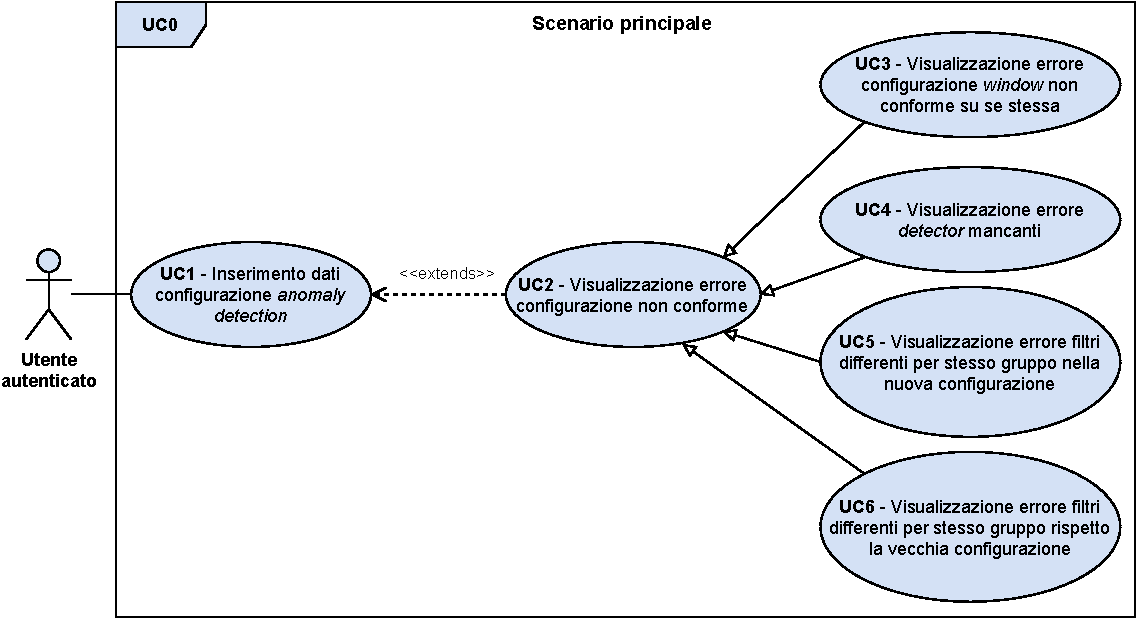
\includegraphics[width=0.9\columnwidth]{usecase/uc0} 
    \caption{Use Case - UC0: Scenario principale}
\end{figure}

\begin{usecase}{0}{Scenario principale}
\usecaseactors{Utente autenticato alla piattaforma \textit{SYN}}
\usecasedesc{Configurazione dei campi richiesti dalla componente di \textit{anomaly detection}}
\usecasepre{L'utente è entrato nella parte della piattaforma relativa alla configurazione dell'\textit{anomaly detection}}
\usecasepost{Il sistema è configurato per rilevare possibili anomalie}
\usecasescenprinc{La finestra visualizzata mette a disposizione una \textit{form} per la compilazione dei campi necessari per la configurazione della componente di \textit{anomaly detection} (\textbf{UC1})}
\usecasealt{La finestra visualizza un messaggio d'errore se i valori inseriti non sono conformi alle attese (\textbf{UC2}), nello specifico vengono visualizzati i seguenti errori:
\begin{itemize}
	\item{la configurazione della \textit{window} non è consistente perchè è presente un gruppo che al suo interno contiene filtri con un \textit{id} non corrispondente a tale gruppo (\textbf{UC3});}
	\item{la configurazione non contiene tutti i \textit{detector} necessari per i gruppi assegnati alla \textit{window} (\textbf{UC4});}
	\item{a parità di gruppo nella nuova configurazione, all'interno della configurazione della \textit{window} e dei \textit{detector}, i filtri risultano essere differenti (\textbf{UC5});}
	\item{a parità di gruppo rispetto la vecchia configurazione, all'interno della configurazione della \textit{window} e dei \textit{detector}, i filtri risultano essere differenti (\textbf{UC6}).}
\end{itemize}}
\label{uc:scenario-principale}
\end{usecase}

\begin{figure}[H] 
    \centering 
    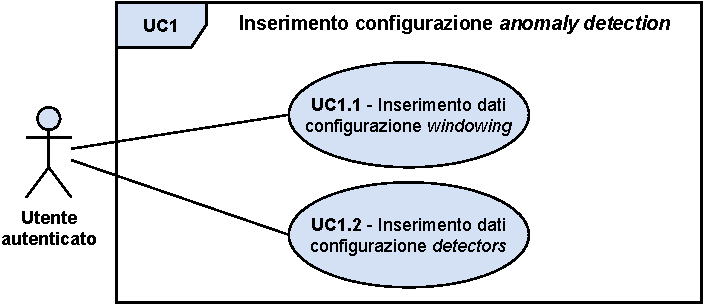
\includegraphics[width=0.9\columnwidth]{usecase/uc1} 
    \caption{Use Case - UC1: Inserimento configurazione \textit{anomaly detection}}
\end{figure}

\begin{usecase}{1}{Inserimento configurazione \textit{anomaly detection}}
\usecaseactors{Utente autenticato alla piattaforma \textit{SYN}}
\usecasedesc{Inserimento dei campi richiesti rispetto la configurazione della \textit{window} e dei \textit{detector}}
\usecasepre{L'utente è entrato nella parte della piattaforma relativa alla configurazione della \textit{window} e dei \textit{detector}}
\usecasepost{I campi relativi alla configurazione della \textit{window} e dei \textit{detector} risultano essere compilati}
\usecasescenprinc{\begin{itemize}
	\item{L'utente inserisce i campi relativi alla configurazione della \textit{window} (\textbf{UC1.1});}
	\item{L'utente inserisce i campi relativi alla configurazione dei \textit{detector} (\textbf{UC1.2}).}
\end{itemize}}
\label{uc:configurazione-anomaly-detection}
\end{usecase}

\section{Classificazione dei requisiti}
I requisiti individuati sono identificati secondo la seguente codifica:
\begin{center}
\textbf{R[Importanza][Tipologia][CodicePadre].\{CodiceFiglio\}}\\
\end{center}
dove:


\begin{itemize}
\item {\textbf{Importanza}: rappresenta l'importanza del requisito e può essere:
	\begin{itemize}
	\item {\textbf{O (Obbligatorio)}: irrinunciabile per garantire il funzionamento richiesto;}
	\item {\textbf{D (Desiderabile)}: non strettamente necessario ma a valore aggiunto riconoscibile;}
	\item {\textbf{F (Facoltativo)}: relativamente utile oppure contrattabile a posteriori nel progetto.}
	\end{itemize}
}
\item{\textbf{Tipologia}: rappresenta il tipo di requisito e può essere:
\begin{itemize}
\item \textbf{F (Funzionale)}: descrive le funzionalità  offerte dall'applicativo;
\item \textbf{V (Vincolo)}: descrive i vincoli che l'applicativo è tenuto a rispettare.
\end{itemize}}
\item \textbf{CodicePadre}: rappresenta il codice di un requisito generico;
\item \textbf{CodiceFiglio} (opzionale): rappresenta il codice di un sotto caso di requisito.
\end{itemize}


\section{Requisiti operatore Bumblebee}
Tale sezione elenca i requisiti Funzionali e di Vincolo individuati per l'operatore \textit{Bumblebee}.
\subsection{Requisiti Funzionali}
{
\centering
\begin{longtable}{L{3cm} L{3cm} L{7.5cm}}
\caption{Requisiti Funzionali dell'operatore \textit{Bumblebee}}\\
\textbf{Identificativo} &
\textbf{Classificazione}&
\textbf{Descrizione}\\
\endhead
\hline

ROF1 & Obbligatorio & L'operatore deve garantire un \textit{output} informativo che possa trattare un \textit{asset} singolo\\
\hline
ROF2 & Obbligatorio & L'operatore deve garantire un \textit{output} informativo che possa trattare un agglomerato di \textit{asset}\\
\hline
ROF2.1 & Obbligatorio & L'operatore deve garantire un \textit{output} informativo che possa trattare un agglomerato di \textit{asset} suddivisi per un gruppo definito dall'utente\\
\hline
\end{longtable}
}

\subsection{Requisiti di Vincolo}
{
\centering
\begin{longtable}{L{3cm} L{3cm} L{7.5cm}}
\caption{Requisiti di Vincolo dell'operatore \textit{Bumblebee}}\\
\textbf{Identificativo} &
\textbf{Classificazione}&
\textbf{Descrizione}\\
\endhead
\hline

ROV1 & Obbligatorio & L'operatore deve garantire un unico tipo di \textit{output} informativo che possa adattarsi alla rappresentazione di \textit{asset} singoli o \textit{asset} agglomerati\\
\hline
\end{longtable}
}





\section{Requisiti operatore Windowing}
Tale sezione elenca i requisiti Funzionali e di Vincolo individuati per l'operatore \textit{Windowing}.
\subsection{Requisiti Funzionali}
{
\centering
\begin{longtable}{L{3cm} L{3cm} L{7.5cm}}
\caption{Requisiti Funzionali dell'operatore \textit{Windowing}}\\
\textbf{Identificativo} &
\textbf{Classificazione}&
\textbf{Descrizione}\\
\endhead
\hline

ROF3 & Obbligatorio & L'operatore deve garantire l'aggregazione di \textit{asset} su se stessi\\
\hline
ROF4 & Obbligatorio & L'operatore deve garantire il raggruppamento di \textit{asset} diversi fra di loro\\
\hline
ROF4.1 & Obbligatorio & L'operatore deve garantire l'aggregazione di \textit{asset} diversi fra di loro\\
\hline
ROF4.2 & Obbligatorio & L'operatore deve garantire l'allineamento di \textit{asset} diversi fra di loro\\
\hline
ROF5 & Obbligatorio & L'operatore deve garantire la creazione di un \textit{output} informativo che rappresenti un'aggregazione degli \textit{asset} su se stessi\\
\hline
ROF6 & Obbligatorio & L'operatore deve garantire la creazione di un \textit{output} informativo che rappresenti un raggruppamento di \textit{asset} differenti\\
\hline
ROF6.1 & Obbligatorio & L'operatore deve garantire la creazione di un \textit{output} informativo che rappresenti un'aggregazione di \textit{asset} differenti fra di loro\\
\hline
ROF6.2 & Obbligatorio & L'operatore deve garantire la creazione di un \textit{output} informativo che rappresenti un allineamento di \textit{asset} differenti fra di loro\\
\hline
ROF7 & Obbligatorio & L'operatore deve garantire la collezione di eventi senza raggruppamento nel caso in cui la finestra temporale sia nulla\\
\hline
ROF8 & Obbligatorio & L'operatore deve garantire la gestione di eventi in anticipo rispetto la finestra temporale attuale\\
\hline
ROF8.1 & Obbligatorio & L'operatore garantisce l'inserimento di eventi in anticipo nella futura finestra temporale se esso è contenuto nei suoi limiti (inizio e fine)\\
\hline
ROF8.2 & Obbligatorio & L'operatore deve scartare eventi in anticipo se essi non sono contenuti nei limiti (inizio e fine) della futura finestra temporale\\
\hline
ROF9 & Obbligatorio & L'operatore deve gestire l'inizio e la fine della prima finestra temporale in base al primo evento ricevuto\\
\hline
ROF10 & Obbligatorio & L'operatore deve collezionare gli eventi relativi alla configurazione in un \textit{output} diverso se questi non sono di tipo "\textit{update}" o "\textit{delete}"\\
\hline
ROF11 & Obbligatorio & L'operatore deve aggiornare la configurazione se questa è diversa da quella precedente o se quella precedente è inesistente\\
\hline
ROF12 & Obbligatorio & L'operatore deve svuotare tutti gli stati se in un evento di configurazione non è presente nessuna configurazione relativa alla finestra temporale\\
\hline
ROF13 & Obbligatorio & L'operatore deve poter creare un \textit{output} di tipo \textit{GroupedEvents} il quale deve essere così formato:
\begin{itemize}
	\item{\textbf{\textit{groupID}:} \textit{id} del gruppo relativo;}
	\item{\textbf{\textit{events}:} \textit{array} di eventi raggruppati o allineati;}
	\item{\textbf{\textit{\textit{\gls{timestamp}}}:} fine della finestra temporale.}
\end{itemize}\\
\hline
ROF13.1 & Obbligatorio & L'operatore deve creare un \textit{output} del tipo \textit{GroupedEvents}, nel caso di allineamento, solo se l'\textit{array} degli eventi risultante non è vuoto\\
\hline
ROF13.2 & Obbligatorio & L'operatore deve creare un \textit{output} del tipo \textit{GroupedEvents}, nel caso di aggregazione, solo se l'evento aggregato ha il campo \textit{DataFields} non vuoto\\
\hline
ROF13.3 & Obbligatorio & L'operatore deve creare un \textit{output} del tipo \textit{GroupedEvents}, nel caso di evento non raggruppato, così formato:
\begin{itemize}
	\item{\textbf{\textit{groupID}:} \textit{id} del gruppo relativo;}
	\item{\textbf{\textit{events}:} \textit{array} contenente solo l'evento entrante;}
	\item{\textbf{\textit{\textit{\gls{timestamp}}}:} \textit{\gls{timestamp}} dell'evento.}
\end{itemize}\\
\hline
ROF14 & Obbligatorio & L'operatore, nel caso di aggregazione di \textit{asset} diversi, deve creare un evento riassuntivo di tutti gli eventi aggregati, il quale verrà inserito come unico elemento all'interno dell'\textit{array} del \textit{GroupedEvents} creato\\
\hline
ROF15 & Obbligatorio & L'operatore, dopo la fine di una finestra temporale, deve poter configurare l'inizio e la fine della futura finestra temporale\\
\hline
ROF16 & Obbligatorio & L'operatore, dopo la fine di una finestra temporale, deve rimuovere gli aggregatori che non contengono eventi futuri per la futura finestra temporale\\
\hline
\end{longtable}
}

\subsection{Requisiti di Vincolo}
{
\centering
\begin{longtable}{L{3cm} L{3cm} L{7.5cm}}
\caption{Requisiti di Vincolo dell'operatore \textit{Windowing}}\\
\textbf{Identificativo} &
\textbf{Classificazione}&
\textbf{Descrizione}\\
\endhead
\hline
ROV2 & Obbligatorio & L'operatore deve garantire un unico tipo di \textit{output} informativo che possa adattarsi alla rappresentazione di \textit{asset} singoli, di \textit{asset} aggregati su se stessi e di \textit{asset} differenti aggregati/allineati fra di loro \\
\hline
ROV3 & Obbligatorio & L'operatore deve garantire che nel caso siano presenti errori riguardanti la struttura di eventi entranti, essi vengano scartati senza provocare l'interruzione del programma\\
\hline
ROV3.1 & Obbligatorio & L'operatore deve scartare gli eventi entranti nel caso essi non contengano le informazioni richieste\\
\hline
ROV3.2 & Obbligatorio & L'operatore deve scartare gli eventi entranti nel caso sia presente un inizio ed una fine di una finestra temporale inconsistente\\
\hline
ROV3.3 & Obbligatorio & L'operatore deve scartare eventi se non è presente nessuna configurazione per la finestra temporale attuale\\
\hline
ROV4 & Obbligatorio & L'operatore deve garantire che, in presenza di errori durante la creazione dell'\textit{output} di tipo \textit{GroupedEvents} alla fine di una finestra temporale, non venga creato tale \textit{output} e che ciò non provochi un'interruzione del programma\\
\hline
ROV4.1 & Obbligatorio & L'operatore non deve creare un \textit{output} di tipo \textit{GroupedEvents} alla fine di una finestra temporale nel caso non sia presente nessuna configurazione di essa\\
\hline
ROV4.2 & Obbligatorio & L'operatore non deve creare un \textit{output} di tipo \textit{GroupedEvents} alla fine di una finestra temporale nel caso sia presente un tipo di \textit{aggregazione} non supportata\\
\hline
RDV1 & Desiderabile & L'operatore deve essere testato per garantire la correttezza della sua operatività\\
\hline
\end{longtable}
}



\section{Requisiti operatore AlertCoProcess}
Tale sezione elenca i requisiti Funzionali e di Vincolo individuati per l'operatore \textit{AlertCoProcess}.
\subsection{Requisiti Funzionali}
{
\centering
\begin{longtable}{L{3cm} L{3cm} L{7.5cm}}
\caption{Requisiti Funzionali dell'operatore \textit{AlertCoProcess}}\\
\textbf{Identificativo} &
\textbf{Classificazione}&
\textbf{Descrizione}\\
\endhead
\hline
ROF17 & Obbligatorio & L'operatore deve riuscire a rilevare anomalie sia su eventi facenti parte di un gruppo sia su eventi non raggruppati\\
\hline
ROF17.1 & Obbligatorio & L'operatore, se opera su un gruppo, deve lanciare l'anomalia su un evento riassuntivo creato per il gruppo\\
\hline
ROF17.2 & Obbligatorio & L'operatore, se opera su un evento singolo, deve lanciare l'anomalia su di esso\\
\hline
ROF18 & Obbligatorio & L'operatore deve creare un nuovo \textit{detector} se esso non è già presente all'interno della mappa dei \textit{detector}\\
\hline
ROF18.1 & Obbligatorio & L'operatore deve creare un nuovo \textit{detector} tramite le informazioni della configurazione se esso è un \textit{LazyLoadDetector}\\
\hline
ROF18.2 & Obbligatorio & L'operatore deve scartare l'evento entrante se il \textit{detector} non è un \textit{LazyLoadDetector} e non è stato trovato\\
\hline
ROF19 & Obbligatorio & L'operatore deve operare tramite \textit{detector} che accettano un singolo \textit{input} o molteplici\\
\hline
ROF20 & Obbligatorio & L'operatore deve supportare la modifica, cancellazione e ispezione della configurazione\\
\hline
ROF21 & Obbligatorio & L'operatore, durante la modifica di una configurazione, deve poter aggiornare la configurazione dei \textit{detector} esistenti, definiti tramite l'\textit{id} del \textit{detector}\\
\hline
ROF21.1 & Obbligatorio & L'operatore, durante la modifica di una configurazione, aggiorna i \textit{detector} tramite la configurazione fornita se si tratta di un \textit{LazyLoadDetector}\\
\hline
ROF21.2 & Obbligatorio & L'operatore, durante la modifica di una configurazione, scarica i \textit{detector} di tipo \textit{LazyLoadDetector} se essi hanno un modello differente da quello salvato (addestrando l'algoritmo di \textit{\gls{Apprendimento automatico}}) \\
\hline
ROF21.3 & Obbligatorio & L'operatore, durante la modifica di una configurazione, crea la futura mappa dei \textit{detector} se non è presente il determinato \textit{id} del \textit{detector} passato dalla configurazione\\
\hline
ROF21.4 & Obbligatorio & L'operatore, durante la modifica di una configurazione, rimuove i \textit{detector} non più richiesti e aggiunge quelli nuovi, aggiornando le rispettive mappe\\
\hline
ROF22 & Obbligatorio & L'operatore, durante la cancellazione di una configurazione, svuota tutti gli stati dell'operatore\\
\hline
ROF23 & Obbligatorio & L'operatore, durante l'ispezione di una configurazione, crea un messaggio riassuntivo dello stato dei \textit{detector} dell'operatore stesso\\
\hline
\end{longtable}
}

\subsection{Requisiti di Vincolo}
{
\centering
\begin{longtable}{L{3cm} L{3cm} L{7.5cm}}
\caption{Requisiti di Vincolo dell'operatore \textit{AlertCoProcess}}\\
\textbf{Identificativo} &
\textbf{Classificazione}&
\textbf{Descrizione}\\
\endhead
\hline
ROV5 & Obbligatorio & L'operatore deve garantire che nel caso siano presenti errori riguardanti la struttura di eventi entranti, essi vengano scartati senza provocare l'interruzione del programma\\
\hline
ROV5.1 & Obbligatorio & L'operatore deve scartare gli eventi su cui verrà rilevata una possibile anomalia se, all'interno della mappa che identifica gli \textit{id} dei \textit{detector}, non è presente la chiave rappresentata dal parametro \textit{groupID} dell'evento di tipo \textit{GroupedEvents} entrante\\
\hline
ROV5.2 & Obbligatorio & L'operatore deve scartare gli eventi su cui verrà rilevata una possibile anomalia se, all'interno della mappa che identifica i \textit{detector}, non è presente la chiave rappresentata come \textit{id} del \textit{detector} estratto dalla mappa contenente tali \textit{id}\\
\hline
ROV5.3 & Obbligatorio & L'operatore deve scartare gli eventi se è richiesto il \textit{detector} di tipo \textit{LazyLoadDetector} e non è stato possibile scaricarlo\\
\hline
ROV5.4 & Obbligatorio & L'operatore deve scartare gli eventi se, operando su un gruppo, è stato richiesto un \textit{detector} che lavora su un singolo \textit{input}\\
\hline
ROV5.5 & Obbligatorio & L'operatore deve scartare l'evento di aggiornamento di un \textit{detector} se esso non contiene l'\textit{id} all'interno del campo \textit{AssetFilters} (\textit{id} identificativo del gruppo)\\
\hline
RDV2 & Desiderabile & L'operatore deve essere testato per garantire la correttezza della sua operatività\\
\hline
\end{longtable}
}

\section{Requisiti API di configurazione}
Tale sezione elenca i requisiti Funzionali e di Vincolo individuati per le \textit{\gls{api}} di governo relative alla configurazione della componente di \textit{anomaly detection}.
\subsection{Requisiti Funzionali}
{
\centering
\begin{longtable}{L{3cm} L{3cm} L{7.5cm}}
\caption{Requisiti Funzionali delle \textit{API} di configurazione}\\
\textbf{Identificativo} &
\textbf{Classificazione}&
\textbf{Descrizione}\\
\endhead
\hline
ROF24 & Obbligatorio & La configurazione fornita dall'\textit{\gls{api}} deve rispecchiare la configurazione attesa dagli operatori\\
\hline
ROF24.1 & Obbligatorio & La configurazione fornita dall'\textit{\gls{api}}, riguardo all'operatore \textit{Windowing}, deve contenere una mappa \textit{assetFilters} dove per chiave è presente l'\textit{id} del gruppo e come valore i filtri applicati ad esso\\
\hline
ROF24.2 & Obbligatorio & La configurazione fornita dall'\textit{\gls{api}}, riguardo all'operatore \textit{AlertCoProcess}, deve contenere un \textit{array} di \textit{detectors}, i quali devono contenere \textit{assetFilters} corrispondenti alla configurazione fornita all'operatore \textit{Windowing}\\
\hline
ROF25 & Obbligatorio & La configurazione relativa all'operatore \textit{Windowing}, per ogni gruppo contenuto all'interno della mappa \textit{assetFilters}, deve avere il relativo valore contenente un \textit{id} eguale alla chiave della mappa\\
\hline
ROF26 & Obbligatorio & Durante la creazione di un nuovo gruppo tramite la configurazione data dall'utente, l'\textit{\gls{api}} deve sostituire l'\textit{id} del gruppo dato, sia nel parametro \textit{windowing.AssetFilters}, che nel parametro \textit{detectors}, con un \textit{id} creato dall'\textit{\gls{api}} stessa\\
\hline
ROF27 & Obbligatorio & Durante la modifica di una configurazione precedente, i gruppi presenti all'interno della nuova configurazione e preesistenti nella precedente configurazione, devono mantenere lo stesso tipo di valore\\
\hline
\end{longtable}
}

\subsection{Requisiti di Vincolo}
{
\centering
\begin{longtable}{L{3cm} L{3cm} L{7.5cm}}
\caption{Requisiti di Vincolo delle \textit{API} di configurazione}\\
\textbf{Identificativo} &
\textbf{Classificazione}&
\textbf{Descrizione}\\
\endhead
\hline
ROV6 & Obbligatorio & L'\textit{\gls{api}} deve fornire un messaggio d'errore all'utente nel caso sia stata fornita una configurazione erronea\\
\hline
ROV6.1 & Obbligatorio & L'\textit{\gls{api}} deve fornire un messaggio d'errore all'utente nel caso sia stata fornita una coppia chiave-valore all'interno del parametro \textit{windowing} cui \textit{valore} non contiene un \textit{id} eguale alla chiave\\
\hline
ROV6.2 & Obbligatorio & L'\textit{\gls{api}} deve fornire un messaggio d'errore all'utente nel caso siano stati forniti, all'interno della configurazione, parametri di \textit{windowing} e \textit{detectors} che non contengono i medesimi gruppi\\
\hline
ROV6.3 & Obbligatorio & L'\textit{\gls{api}} deve fornire un messaggio d'errore all'utente nel caso sia fornito una configurazione contenente gruppi preesistenti nella configurazione precedente, ma con differente lista di valori\\
\hline
RDV3 & Desiderabile & L'\textit{\gls{api}} deve essere testata per garantire la correttezza della sua operatività\\
\hline
\end{longtable}
}


\section{Tracciamento requisiti - ambito di sviluppo}
{
\centering
\begin{longtable}{L{5cm} L{8.5cm}}
\caption{Tracciamento requisiti - ambito di sviluppo}\\
\textbf{Identificativo requisito} &
\textbf{Ambito di sviluppo}\\
\endhead
\hline

ROF1 \newline ROF2 \newline ROF2.1 \newline ROV1 & Operatore \textit{Bumblebee} \\
\hline
ROF3\newline ROF4 \newline ROF4.1 \newline ROF4.2 \newline ROF5 \newline ROF6 \newline ROF6.1 \newline ROF6.2 \newline ROF7 \newline ROF8 \newline ROF8.2 \newline ROF9 \newline ROF10 \newline ROF11 \newline ROF12 \newline ROF13 \newline ROF13.1 \newline ROF13.2 \newline ROF13.3 \newline ROF14 \newline ROF15 \newline ROF16 \newline ROV2 \newline ROV3 \newline ROV3.1 \newline ROV3.2 \newline ROV3.3 \newline ROV4 \newline ROV4.1 \newline ROV4.2 \newline RDV1 & Operatore \textit{Windowing} \\
\hline
ROF17 \newline ROF17.1 \newline ROF17.2 \newline ROF18 \newline ROF18.1 \newline ROF18.2 \newline ROF19 \newline ROF20 \newline ROF21 \newline ROF21.1 \newline ROF21.2 \newline ROF21.3 \newline ROF21.4 \newline ROF22 \newline ROF23 \newline ROV5 \newline ROV5.1 \newline ROV5.2 \newline ROV5.3 \newline ROV5.4 \newline ROV5.5 \newline RDV2 & Operatore \textit{AlertCoProcess} \\
\hline
ROF24 \newline ROF24.1 \newline ROF24.2 \newline ROF25 \newline ROF26 \newline ROF27 \newline ROV6 \newline ROV6.1 \newline ROV6.2 \newline ROV6.3 \newline RDV3 & \textit{\gls{api}} di configurazione \\
\hline
\end{longtable}
}